Gang er en fysisk bevægelse, som benytter involverer hele kroppen til at koordinere bevægelsen. Den følgende beskrivelse af én gangcyklus, tager udgangspunkt i beskrivelsen af bevægelserne for det højre ben. Bevægelserne er dog tilsvarende for det venstre ben. \citep{VaughanDavisOConnor1992,Whittle1990}

En gangcyklus begynder når den højre fod har opnået kontakt med underlaget. Når denne cyklus er påbegyndt, inddeles cyklussen endvidere i to faser; standfasen og svingfasen, hvilket fremgår af \figref{fig:gang_cyklus}. \newline
Standfasen har en varighed svarende til cirka 60\% af en gangcyklus. Dette skyldes, at standfasen indebærer den tid hvor højre fod er i berøring med jorden. Derimod er svingfasen blot en fase på cirka 30\% af hele gangcyklussen. \citep{VaughanDavisOConnor1992} Svingfasen er dermed den varighed, hvor foden og benet bevæges frem og er derfor ikke i berøring med jorden. Denne fod klargører dermed til den kommende kontakt med jorden, foran den venstre fod som er i berøring med underlaget.

\begin{figure}[H]
	\centering
	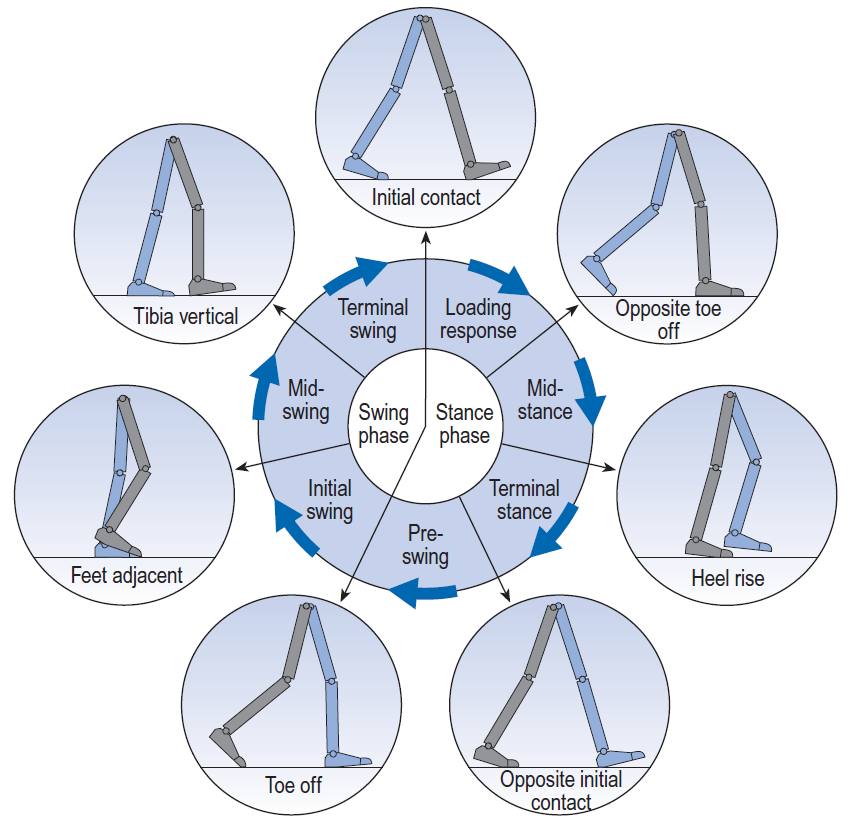
\includegraphics[scale=0.5]{figures/bProblemloesning/gang_cyklus2.png}
	\caption{Figurtekst… \fxnote{SKAL MODIFICERES. Gør så at figuren også har den procentvise fordeling af faserne på} \cite{VaughanDavisOConnor1992}}
	\label{fig:gang_cyklus}
\end{figure}

Det fremgår af billedet, at standfasen og svingfasen yderligere er inddelt henholdsvis i 5 og 3 faser. \newline
Standfasen første fase er et hæl-nedslag som starter hele cyklussen, idet der opnås kontakt med overfladen med den højre hæl. Herefter er foden flad og den venstre fod er derimod i berøring med overfladen med tåspidserne. Hælen på den højre fod løftes nu, alt i mens den venstre fod, som er i svingfasen, passerer den højre fod. Der opstår nu et hæl-slip for den højre fod, og der skabes en berøring af den venstre fod på underlaget. Standfasen afsluttes med en fleksion af anklen og dermed et afsæt fra tæerne på højre fod. \newline
Den højre fod, og det højre ben, er dermed i svingfasen, som påbegyndes med en acceleration af foden og benet. Denne acceleration begynder når foden ikke længere har kontakt med underlaget i standfasen. Derfor vil det højre ben blive bevæget frem mod det venstre ben. Efterfølgende vil der være et såkaldt, midt-sving som forekommer når højre fod er lige under kroppen og dermed ud for den venstre fod, som er i kontatkt med jorden. Afsluttende for svingfasen er der en deacceleration. Denne fase involverer en række muskler som sænker hastigheden af benet og fodens fremadgående bevægelse, således kroppen er klar til det kommende hæl-nedslag i standfasen.






